\documentclass[tikz,border=10pt]{standalone}
\usepackage{tikz, pgfplots}
\pgfplotsset{compat=1.18}

% Define labels for glossary terms
\newcommand{\pcnc}{PCNC}
\newcommand{\fc}{FC}

\begin{document}

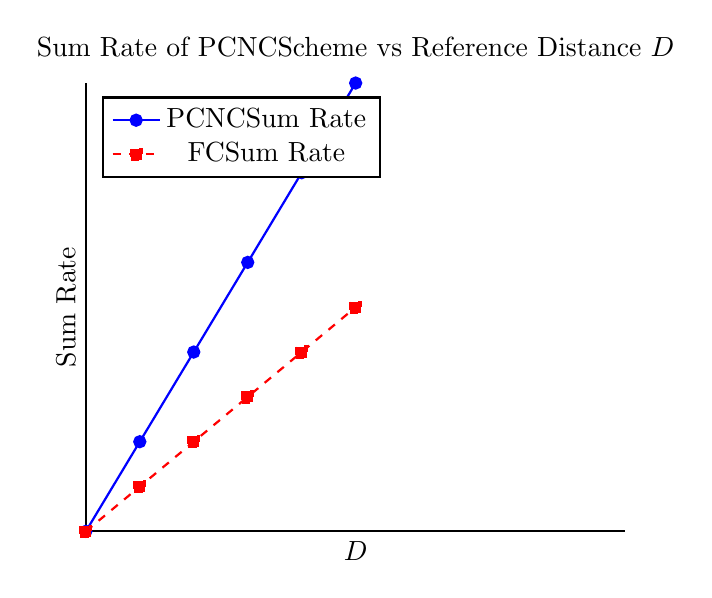
\begin{tikzpicture}
    \begin{axis}[
        title={Sum Rate of \pcnc Scheme vs Reference Distance $D$},
        xlabel={$D$},
        ylabel={Sum Rate},
        legend entries={\pcnc Sum Rate, \fc Sum Rate},
        legend pos=north west,
        grid=major,
        xmin=0, xmax=10,
        ymin=0, ymax=10,
        xtick=\empty,
        ytick=\empty,
        axis lines*=left,
        every tick label/.append style={font=\tiny},
        thick
    ]
        
        % Plot the PCNC sum rate
        \addplot[blue, mark=*] coordinates {
            (0, 0)
            (1, 2)
            (2, 4)
            (3, 6)
            (4, 8)
            (5, 10)
        };
        \label{plot:pcnc_sum_rate}
        
        % Plot the FC sum rate (dashed line)
        \addplot[dashed, red, mark=square*] coordinates {
            (0, 0)
            (1, 1)
            (2, 2)
            (3, 3)
            (4, 4)
            (5, 5)
        };
        \label{plot:fc_sum_rate}
        
    \end{axis}
\end{tikzpicture}

\end{document}